\documentclass[a4paper, 10pt]{article}

\usepackage[margin = 1in]{geometry} % for spacing around
\usepackage{graphicx} % for including images in your pdfs
\usepackage{xcolor} % for including colors in your pdf
\usepackage{soul} % for text decoration
\usepackage[utf8]{inputenc} % for encoded text
\usepackage[T1]{fontenc}
\usepackage{setspace} % for setting different line spacings between paragrafs.
\usepackage{enumerate} % for letting us get more detailed enumerate lists
\usepackage{multirow} % to let us combine more rows together
\usepackage{colortbl} % for decorating tables
\usepackage{amsmath} % used for representing more complicated math displays
\usepackage{supertabular}
\usepackage{longtable} % both of these packages are used to making really big tables
\usepackage{wrapfig} % allows us to wrap text around figures
\usepackage{fancyhdr} % for making fancy headers
%\usepackage{bibtex} % for making better bibliographies
\usepackage[pdftex]{hyperref} % for letting us make links
\usepackage{lscape} % Allows us to flip from portrait to landspace
\usepackage{tikz} % for high detailed drawing
\usepackage{multicol} % To put things side by side
\usepackage{rotating} % For rotating objects
% \usepackage{draftwatermark} % For adding watermarks
\usepackage{MnSymbol} % for using multiple symbols
\usepackage{mathtools} % Used for more math symbols
\usepackage{xfrac} % For more complciated fractions and to add derivitives
\usepackage{hyperref} % for hyper links
\usepackage{enumitem} % for better enum lists
\usepackage{tcolorbox} % for adding colored text boxes
\usepackage{bm} % Adding bold text to math inputs
\usepackage{pgfplots} % Used for plotting functions
\pgfplotsset{compat=1.18}
\usepackage[siunitx]{circuitikz} % For drawing circuits
\usepackage{caption} % For adding captions to images
\usepackage{siunitx} % Add this line to import the siunitx package
\usepackage{booktabs} % For prettier tables

% Setting up the default image path
\graphicspath{{../../global-assets/images/}}

% Implementing authro details
\title{Lab Report number I - Title of the lab report\\
	ENS203 - Electrical Circuits I}
\author{Emre Arapcic-Uevak\\220302289}
\date{}

% Setting up the fancy page style
\fancypagestyle{customStyle}{
	\lhead{} \chead{} \rhead{}
	\lfoot{} \cfoot{\thepage} \rfoot{}
	\renewcommand{\headrulewidth}{0pt}
	\renewcommand{\footrulewidth}{1pt}
}
\pagestyle{customStyle}

% Custom commands


\begin{document}
	\begin{titlepage}
		\begin{center}
			\vspace*{\stretch{1}} % Add vertical space before the title

			{\Large\bfseries Lab Report number 3 \\[0.5em] Series / Parallel Circuits\par}
			\vspace{1cm} % Space between title and course title

			{\large ENS203 – Electrical Circuits I\par}
			\vspace{1cm} % Space between course title and your name/ID

			{\large Emre Arapcic-Uevak \\ 220302289\par}
			\vspace{.3cm} % Space between your name/ID and assistant name
			{\large Afan Haznadarevic \\ 220302128\par}
			\vspace{1cm} % Space between your name/ID and assistant name

			{\large Assistant: Adil Hasanbasic\par}
			\vspace{\stretch{2}} % Variable vertical space between assistant name and bottom
			
\includegraphics[width=0.5\textwidth]{Logo.png}
			\vspace{5mm}
			
			\textsc{\LARGE Internation University of Sarajevo}\\[1.5cm]
			\textsc{\Large ENS203 - Electrical Circuits I}\\[0.5cm]
			
			\rule{\linewidth}{0.5mm} \\[0.4cm]
			{ \huge \bfseries Lab Report number III - Series / Parallel Circuits}\\[0.4cm]
			\rule{\linewidth}{0.5mm} \\[1.5cm]
			
			\vfill
			
			% Bottom of the page
			{\large \today}
		\end{center}
	\end{titlepage}
	\pagebreak

	\tableofcontents
	\pagebreak
	
	\listoffigures
	\pagebreak
	
	\section{Objective}
		The objective of this lab is to understand Kirchhoff's laws and how they can be applied to series and parallel circuits.
		We will build three different circuits in this lab and try to show the validity of Kirchhoff's laws.
		
		\subsection{Kirchhoff's Laws}
			\begin{itemize}
				\item Kirchhoff's Current Law (KCL): The sum of currents entering a node is equal to the sum of currents leaving the node.
				\item Kirchhoff's Voltage Law (KVL): The sum of voltages around a closed loop is equal to zero.
			\end{itemize}
	
		\subsection{Equipment}
			\begin{itemize}
				\item Breadboard
				\item Resistors 1\si{\kilo\Omega}, 10 \si{\kilo\Omega}, 100 \si{\Omega}
				\item 1 LED
				\item DC Power supply
				\item Multimeter
			\end{itemize}

			\subsubsection{Breadboard}
				A breadboard is a construction base for prototyping of electronics.A breadboard consists of plastic block holding a matrix of electrical sockets of a size suitable for gripping thin connecting wire, 
				component wires or the pins of transistors and integrated circuits (ICs). The sockets are connected inside the board, usually in rows of five sockets.

				\begin{figure}[h!]
					\centering
					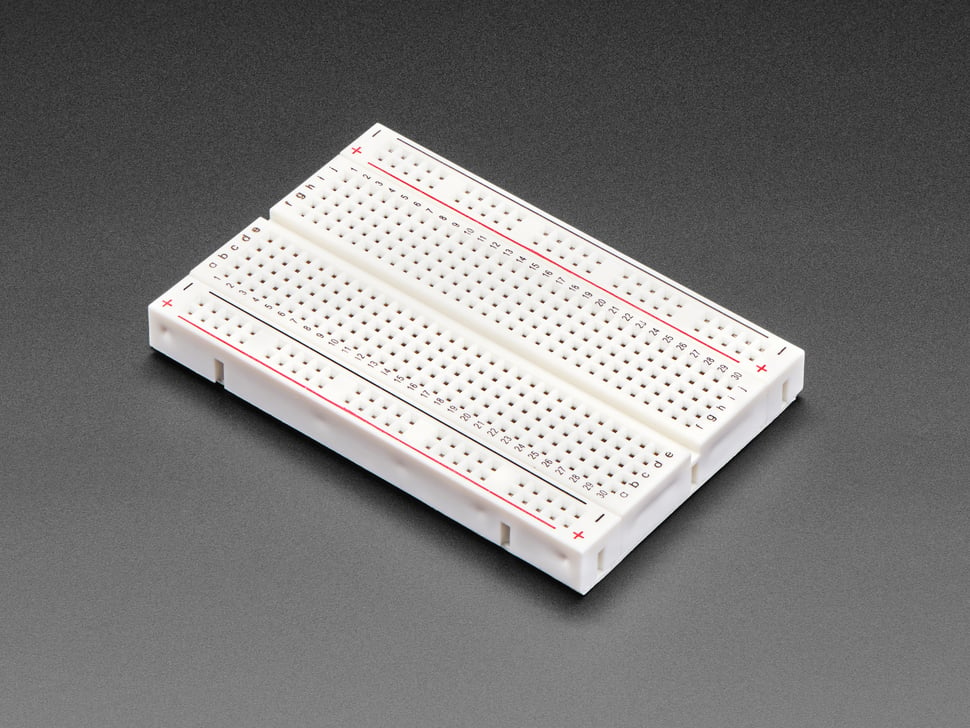
\includegraphics[width=0.5\textwidth]{images/breadboard.jpeg}
					\caption{A breadboard}
					\label{fig:breadboard}
				\end{figure}
			

			\pagebreak

			\subsubsection{Resistors}
				As stated before we needed 3 resistors for this lab report so we took 3 resistors with the proper colour code values and then we measured them and marked them.

				\begin{figure}[h!]
					\centering
					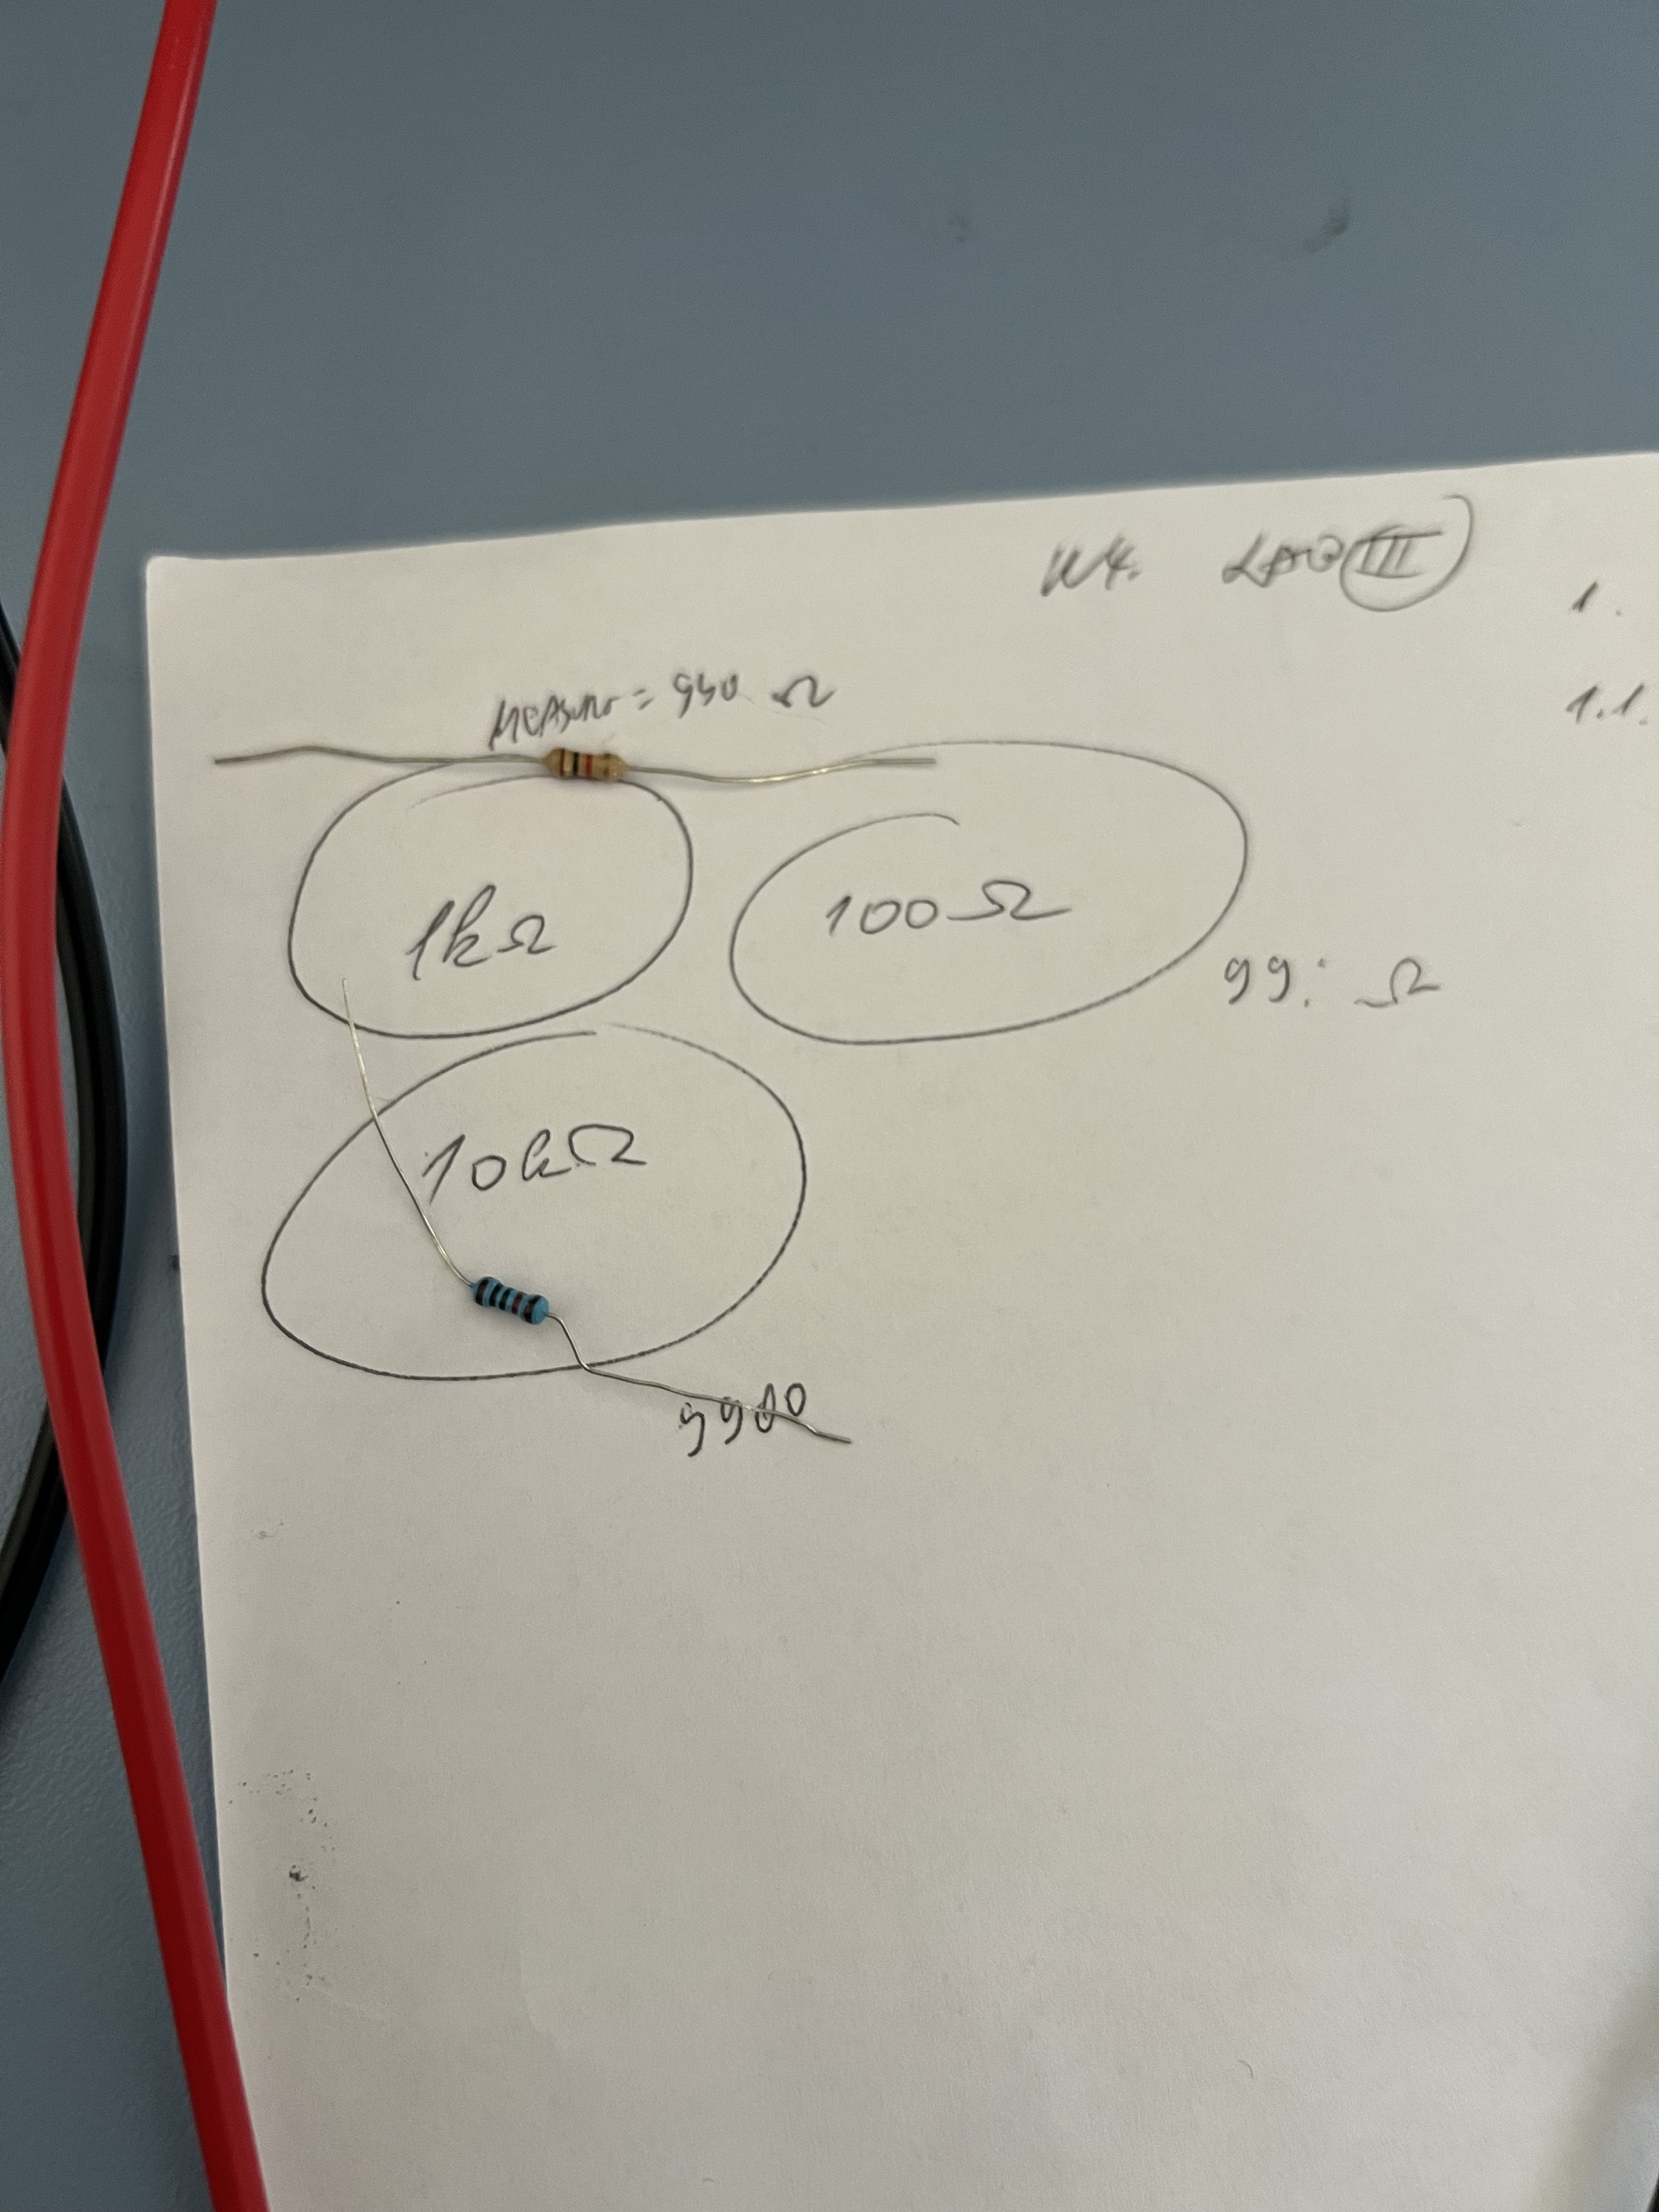
\includegraphics[width=0.35\textwidth]{images/Resistors.jpeg}
					\caption{Resistors with their measured values}
					\label{fig:resistors}
				\end{figure}

	
				\begin{table}[h!]
					\centering
					\begin{tabular}{@{}l|S|S@{}} % l for left, S for siunitx number column
						\toprule
						{Resistor} & {Expected Value (\si{\ohm})} & {Measured Value (\si{\ohm})} \\
						\midrule
						R1 & 100 & 99 \\
						R2 & 1000 & 990 \\
						R3 & 10000 & 9900 \\
						\bottomrule
					\end{tabular}
					\caption{Expected and Measured Resistance Values}
					\label{tab:resistors}
				\end{table}

			\subsubsection{LED}
				An LED (Light Emitting Diode) is a semiconductor device that emits light when an electric current passes through it. LEDs are commonly used in electronic circuits for various purposes, such as indicator lights, displays, and illumination.
				In this lab, a red LED was used. Red LEDs emit red light with a specific wavelength. They are widely used in applications such as traffic lights, electronic displays, and decorative lighting.
				Here is an image of a red LED:

				\begin{figure}[h!]
					\centering
					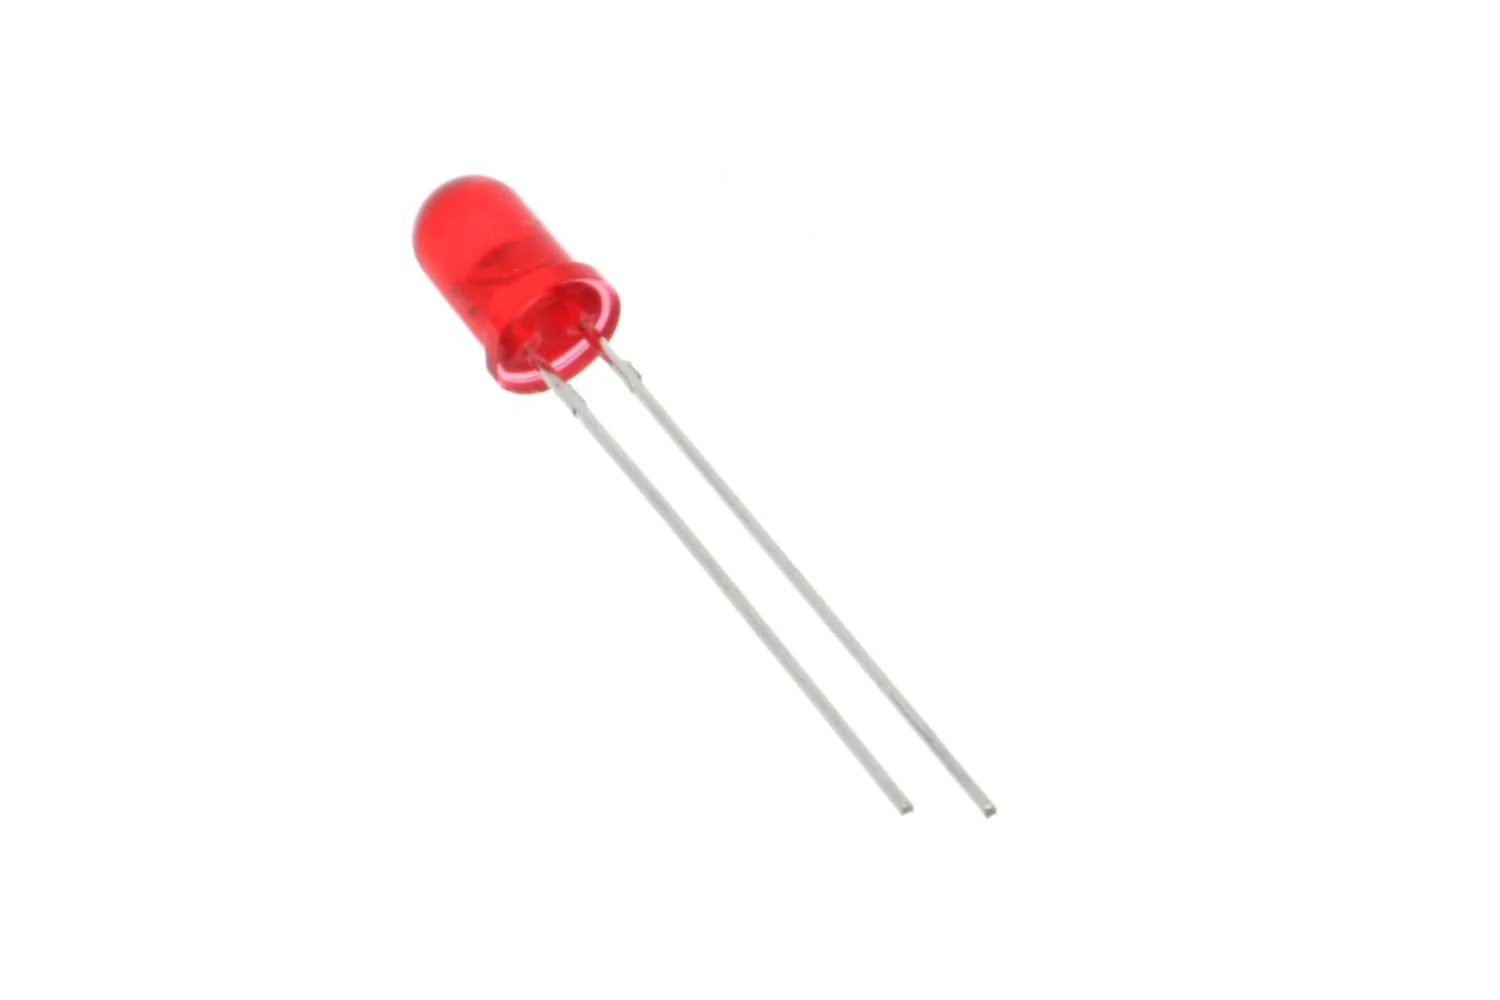
\includegraphics[width = 0.5\textwidth]{images/LED.jpeg}
					\caption{Red LED}
					\label{fig:red_led}
				\end{figure}

			\pagebreak

			\subsubsection{Multimeter}
				The multimeter is a versatile tool used for measuring various electrical quantities. In this lab, we will use it to measure the voltage drops across components, the currents through branches and components, and the resistance of resistors.
				To measure voltage drops, connect the multimeter in parallel across the component of interest. Set the multimeter to the voltage measurement mode and select an appropriate range.
				To measure currents, connect the multimeter in series with the branch or component. Set the multimeter to the current measurement mode and select an appropriate range.
				To measure resistance, disconnect the resistor from the circuit. Connect the multimeter probes to the resistor terminals. Set the multimeter to the resistance measurement mode and select an appropriate range.

				\begin{figure}[h!]
					\centering
					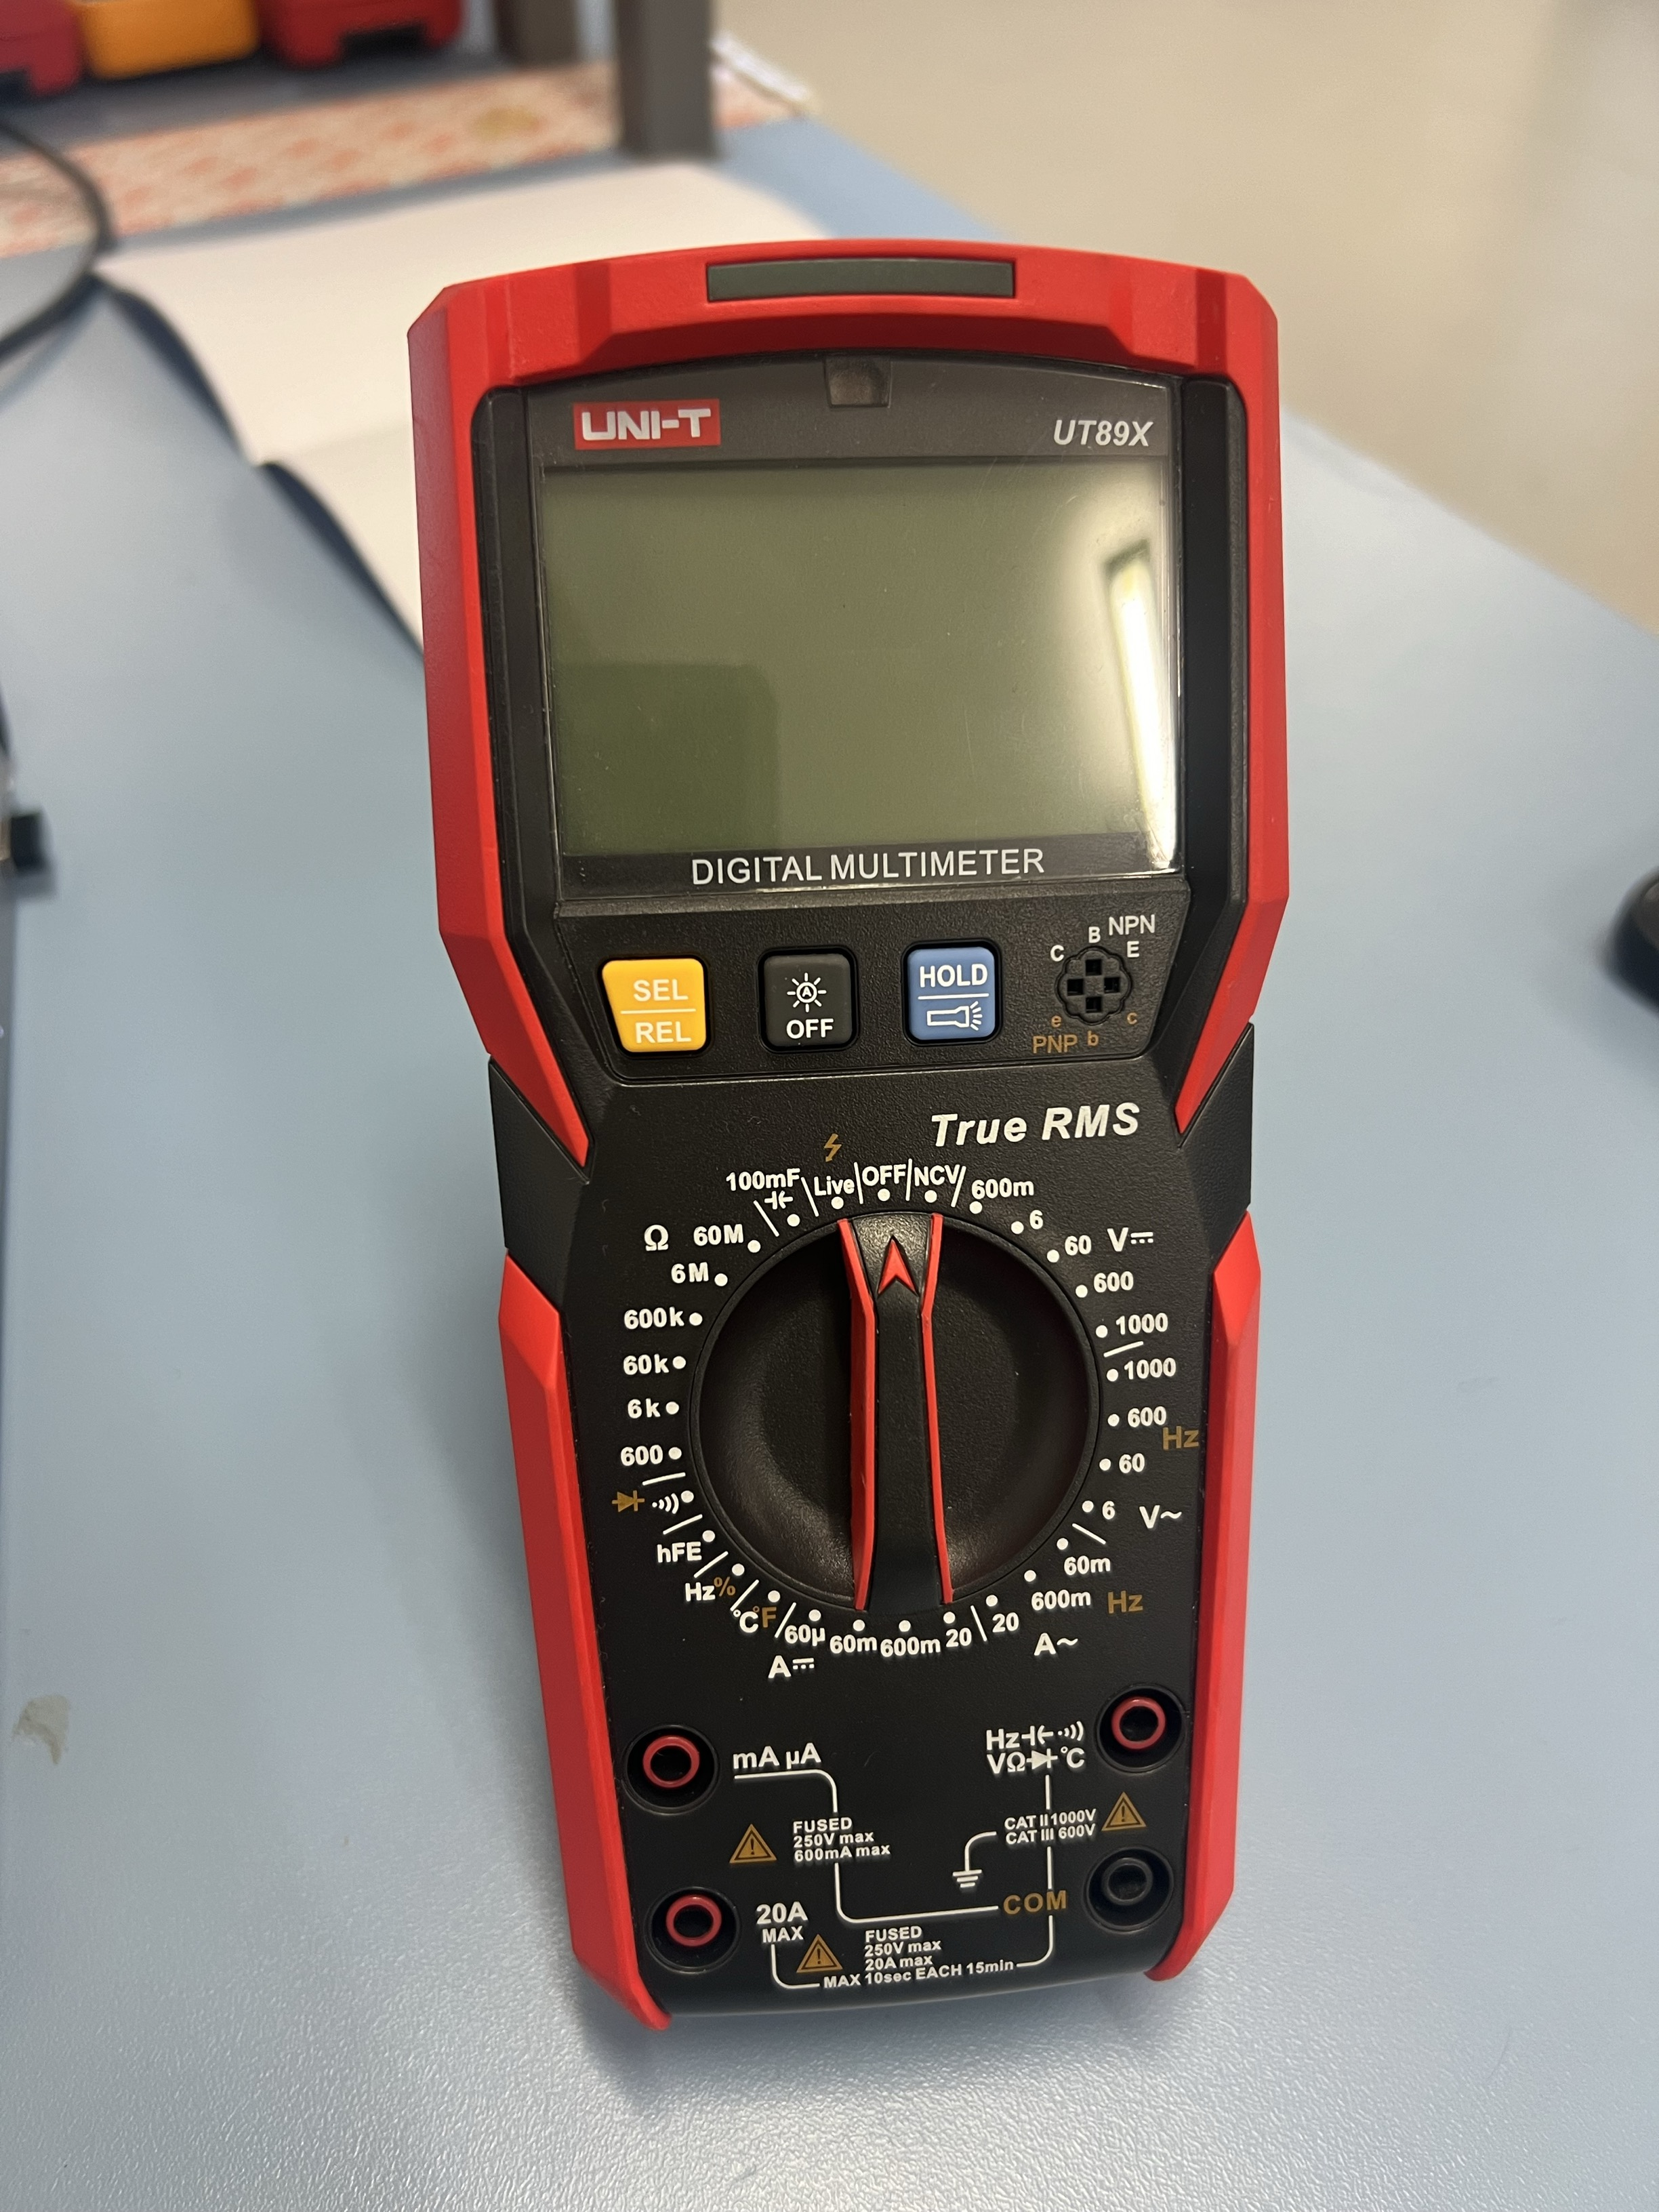
\includegraphics[height = 0.3\textheight]{images/Multimeter.jpeg}
					\caption{Multimeter}
					\label{fig:multi_meter}
				\end{figure}

	\pagebreak
	\section{Circuit 1}
		\begin{figure}[h!]
			\centering
			\begin{circuitikz}[line width=0.75pt]
				\draw
				(0,0) to[V, V=\SI{5}{\volt}, invert, fill=green!50] ++(0,3) % Voltage source
				to[R, l=\SI{100}{\ohm}, fill=red!50] ++(3,0)              % Resistor
				to[led, fill=red!50] ++(0,-3)                              % LED
				-- (0,0);                                                   % Connection back to the beginning
				% Adding an arrow to emphasize voltage drop across the LED
				\draw[<->, >=stealth, thick, blue] (3.9,2) -- node[right] {Voltage drop} (3.9,0.95);
			  \end{circuitikz}
			\caption{Simple LED circuit with a 5V power supply and a 100 ohm resistor.}
			\label{fig:simple_led_circuit}
		\end{figure}

		\subsection{Objectives}
			\begin{itemize}
				\item To measure the voltage drop across the LED.
				\item To measure the voltage drop across the resistor.
				\item Ensure that the sum of the voltage drops is equal to the voltage of the power supply, hence validating Kirchhoff's Voltage Law.
			\end{itemize}

		\subsection{Making the circuit}
			
\end{document}
